%%%%%%%%%%%%%%%%%%%%%%%%%%%%%%%%%%%%%%%%%%%%%%%%%%%%%%%%%%%%%%%%%%%%%%
% Source: http://www.howtotex.com
%%%%%%%%%%%%%%%%%%%%%%%%%%%%%%%%%%%%%%%%%%%%%%%%%%%%%%%%%%%%%%%%%%%%%%
\documentclass[paper=a4, fontsize=11pt]{scrartcl}
\usepackage[T1]{fontenc}
\usepackage{fourier}

%\usepackage{minted}
%\usemintedstyle{cpp}
%\usemintedstyle{trac}
%\newminted{cpp}{bgcolor=col, linenos=true}


\usepackage{siunitx}

\usepackage{xcolor}
\usepackage[pdftex]{graphicx}  
\usepackage[]{minted}
\setminted{linenos,bgcolor=col, obeytabs=true}
\definecolor{col}{rgb}{0.85,0.85,0.85}
%\BeforeBeginEnvironment{minted}{\begin{tcolorbox}}%
%\AfterEndEnvironment{minted}{\end{tcolorbox}}%

\usepackage[english]{babel}                                                                                                                     % English language/hyphenation
\usepackage[protrusion=true,expansion=true]{microtype}  
\usepackage{amsmath,amsfonts,amsthm} % Math packages
\newcommand*{\rttensor}[1]{\overline{\overline{#1}}}
\newcommand{\pfrac}[2]{\frac{\partial#1}{\partial#2}}



\usepackage{algpseudocode,algorithm2e}
\usepackage{url}
\usepackage{hyperref}


\usepackage[numbers]{natbib}
%\usepackage[style=ieee]{biblatex}

%%% Custom sectioning

\usepackage{sectsty}
\allsectionsfont{\centering \normalfont\scshape}


%%% Custom headers/footers (fancyhdr package)
\usepackage{fancyhdr}
\pagestyle{fancyplain}    
\fancyhead{}% No page header
\fancyfoot[L]{}% Empty 
\fancyfoot[C]{}% Empty
\fancyfoot[R]{\thepage}% Pagenumbering
\renewcommand{\headrulewidth}{0pt}% Remove header underlines
\renewcommand{\footrulewidth}{0pt}% Remove footer underlines
\setlength{\headheight}{10.6pt}


%%% Equation and float numbering
\numberwithin{equation}{section}                % Equationnumbering: section.eq#
\numberwithin{figure}{section}                  % Figurenumbering: section.fig#
\numberwithin{table}{section}                           % Tablenumbering: section.tab#


%%% Maketitle metadata
\newcommand{\horrule}[1]{\rule{\linewidth}{#1}}         % Horizontal rule

\title{%\vspace{-1in}      
    \usefont{OT1}{bch}{b}{n}
    \normalfont\normalsize \textsc{Kevin T. Crofton Department of Aerospace and Ocean Engineering} \\ [25pt]
    \horrule{0.5pt} \\[0.4cm]
    \huge Magneto Rayleigh-Taylor Instability for an Annulus using Finite Volume Method with the MagnetoHydroDynamic Equations  \\
    \horrule{2pt} \\[0.5cm]}
\author{\normalfont\normalsize
  Robert Masti\\[-3pt]  
  \normalsize\today}
\date{}


%%% Begin document
\begin{document}
\maketitle
\section{MRT Overview \& Simulation Setup}\label{sec:ovrvw}
The magneto Rayleigh-Taylor instability (MRT) occurs when there is a heavy fluid supported by a light fluid under the influence of gravity with the addition of magnetic fields. Depending on the orientation of these magnetic fields they can have stabilizing characteristics for the growth of this instability. MRT being a hydrodynamic instability means it can be moduled using the ideal MagnetoHydroDynamic (MHD) equations with fluid modeling. This instability is one of the most detrimental instabilities in the plasma communities attempting to reach nuclear fusion ignition. This study analyzed a configuration for a specific nuclear fusion concept known as Direct Drive. The Direct Drive inertial confinement fusion concept uses direct application of lasers onto a spherical shell that implodes through shell ablation. This concept is currently being explored at the National Ignition Facility, and Figure~\ref{fig:ovrvw:dd} depicts this in further detail. The densities, pressures, and acceleration are taken from \href{https://www.astro.princeton.edu/~jstone/Athena/tests/rt/rt.html}{Athena Webpage} for implememntation purposes, but transition to realistic densities, pressures, and acceleration is the goal.


  \begin{figure}[!htb]
    \centering
    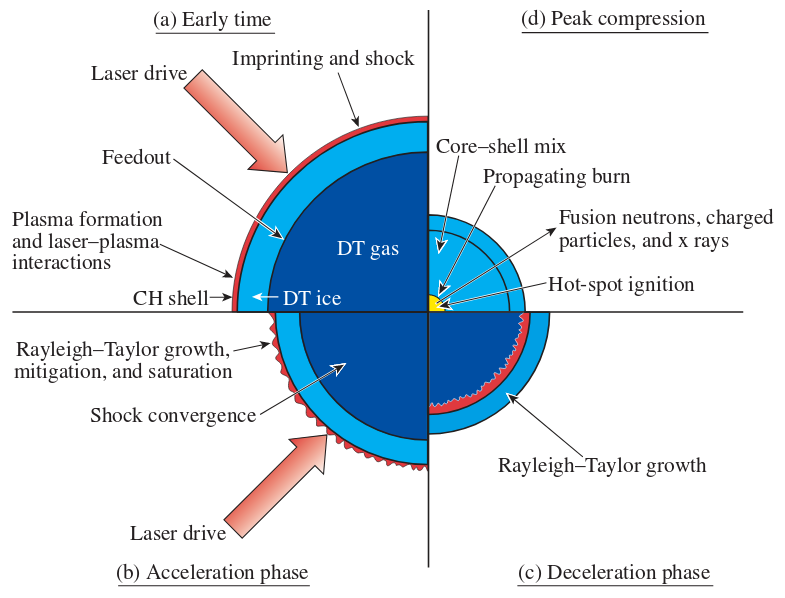
\includegraphics[width=0.9\linewidth]{fig/DDfusion}
    \caption{Shows the four main stages during a typical direct-drive target implosion.\cite{craxton2015}}\label{fig:ovrvw:dd}
  \end{figure}

\subsection{MHD Equation System}

The MHD equations allow for the incorporation of electric and magnetic fields as they influence a conducting medium. It has the continuity, conservation of momentum, and energy, like in Euler equations, but it has the addition of an induction equation for the magnetic field. In a plasma there is co existing electrons and ions, and in MHD limit the electron fluid equations are used to derive the electric field used in the induction equation, and the extent of this electric field can be extended or retracted to incorporate more or less electron physics into the equation system. Initially just the Lorentz force term will be used as the electric field contribution to the induction equation. Assuming ideal gas EOS the MHD equations are given by

\minipage{\textwidth}
  \minipage{0.48\textwidth}
  \begin{align*}
    \pfrac{\rho}{t} + \nabla \cdot \left[\rho \mathbf{u}\right] &= 0 \\
    \pfrac{\rho \mathbf{u}}{t} + \nabla \cdot \left[\rho \mathbf{u}\mathbf{u}^T - \mathbf{b}\mathbf{b}^T + \mathbb{I}\left(P + \frac{1}{2}|\mathbf{b}|^2\right)\right] &= 0 \\
    \pfrac{\epsilon}{t} + \nabla \cdot \left[\left(\epsilon + P + \frac{1}{2}|\mathbf{b}|^2\right)\mathbf{u}- \mathbf{b}\cdot\mathbf{u}\mathbf{b}\right] &= 0 \\
    \pfrac{\mathbf{b}}{t} + \nabla\times\mathbf{e} &= 0 \\
  \end{align*}
  \endminipage\hfill
  \minipage{0.48\textwidth}
  \begin{align*}
    \mathbf{b} &= \frac{\mathbf{B}}{\sqrt{\mu_0}} \\
    \mathbf{e} &= - \mathbf{u} \times \mathbf{b} +\left(\mathbf{e}^{external}\rightarrow\mathbf{0}\right)\\
    \epsilon &= \epsilon_{internal} + \frac{1}{2}\rho|\mathbf{u}|^2 + \frac{1}{2}|\mathbf{b}|^2\\
    P &=\rho \epsilon_{internal} (\gamma - 1) \\
  \end{align*}
  \endminipage\hfill
  \endminipage, where $\rho$, $\mathbf{u}$, $\mathbf{e}$, $\mathbf{b}$, $P$, $\gamma$, $\epsilon$, and $\mu_0$ are density, velocity, electric field, magnetic field, pressure, adiabatic gas constant, specific internal energy, and magnetic permeability of free space, respectively. In this equation system there is no externally applied electric fields ($e.q.\;\eta \mathbf{j}$). The equation for the magnetic field must be manipulated with vector identities into a divergence form through
  \begin{align*}
    \pfrac{\mathbf{b}}{t} + \nabla\times(-\mathbf{u}\times\mathbf{b}) &= 0\\
    \pfrac{\mathbf{b}}{t} - \left[\mathbf{u}(\nabla\cdot\mathbf{b})-\mathbf{b}(\nabla\cdot\mathbf{u})+(\mathbf{b}\cdot \nabla)\mathbf{u}-(\mathbf{u}\cdot\nabla)\mathbf{b}\right] &= 0\\
    \pfrac{\mathbf{b}}{t} - \left[\nabla\cdot(\mathbf{b}\mathbf{u}^T)-\nabla\cdot(\mathbf{u}\mathbf{b}^T)\right] &= 0\\
    \pfrac{\mathbf{b}}{t} + \nabla\cdot\left[\mathbf{u}\mathbf{b}^T-\mathbf{b}\mathbf{u}^T\right] &= 0\\
  \end{align*}, and this can be used to rewrite the equation system into a tensor product form given by 
\begin{equation}\label{eqn:mhdvector}
  \pfrac{\mathbf{Q}}{t} + \nabla \cdot \rttensor{T} = 0
\end{equation}
where $\mathbf{Q}$ is the conserved variables vector, and $\rttensor{T}$ is the flux tensor. $\mathbf{Q}$, and $\rttensor{T}$, are given by
\[
  \mathbf{Q}=
  \begin{bmatrix}
    \rho  \\
    \rho \mathbf{u}  \\
    \epsilon\\
    \mathbf{b} 
  \end{bmatrix}
  ,\quad \rttensor{T} =
  \begin{bmatrix}
    \rho \mathbf{u}  \\
    \rho \mathbf{u}\mathbf{u}^T - \mathbf{b}\mathbf{b}^T + \mathbb{I}\left(P + \frac{1}{2}|\mathbf{b}|^2\right)\\
    \left(\epsilon + P + \frac{1}{2}|\mathbf{b}|^2\right)\mathbf{u}- \mathbf{b}\cdot\mathbf{u}\mathbf{b}\\
    \mathbf{u}\mathbf{b}^T-\mathbf{b}\mathbf{u}^T
  \end{bmatrix}
\]
, respectively. 



\subsection{Discretization \& Flux Formulation}\label{sec:disc}
  \begin{figure}[!htb]
    \centering
    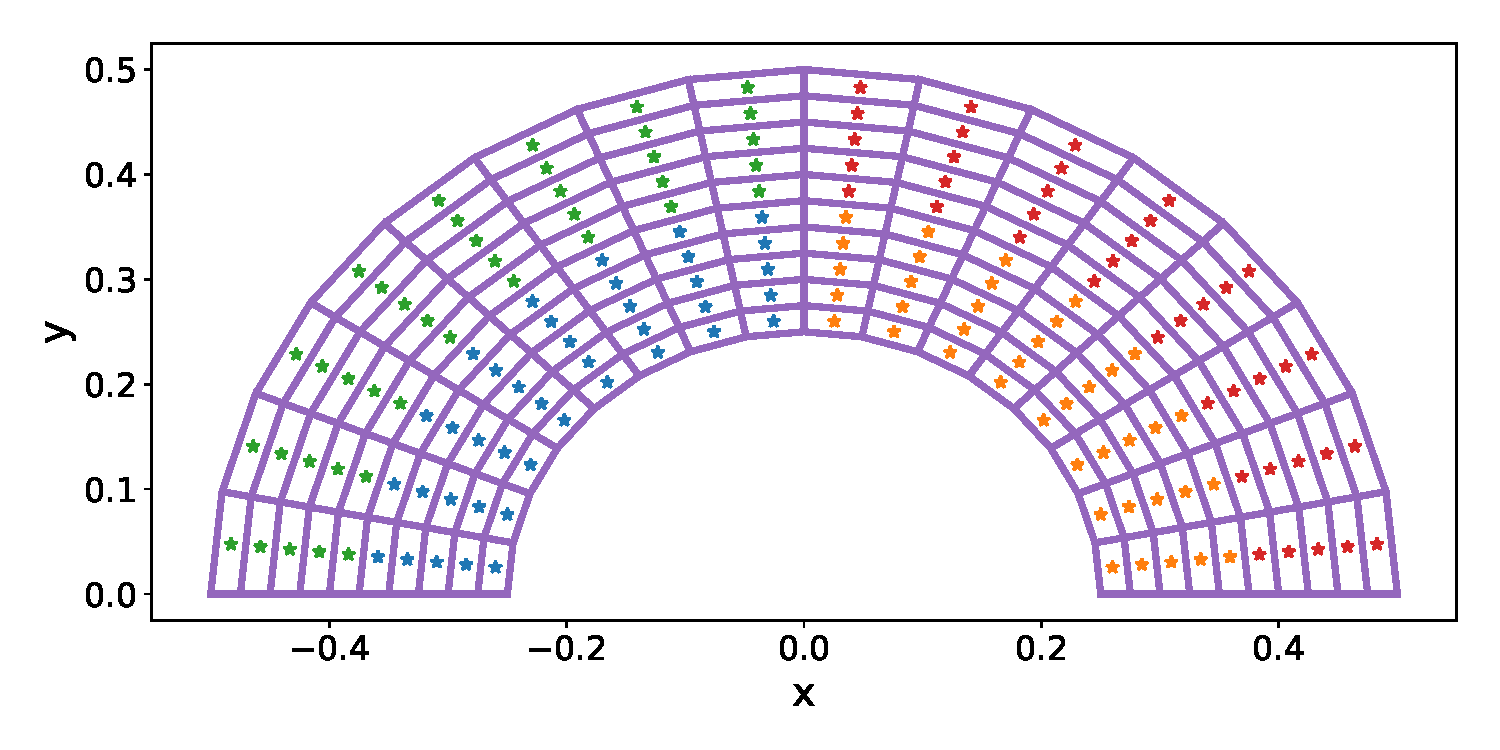
\includegraphics[width=1.0\linewidth]{fig/16x10mesh.pdf}
    \caption{A mesh example using 16 cells in the i direction and 10 cells in the j direction with cell centers highlighted using 4 partitions}\label{fig:ovrvw:mesh}
  \end{figure}

The simulation setup will use a discretization shown in Figure~\ref{fig:ovrvw:mesh} where the coordinates are unitless currently with the mesh generation being done in MATLAB for this simplistic geometry. In order to evaluate the flux in the x and y direction the normal vectors on the cell faces are required. With the normal vectors and areas known the fluxes can be determined for MHD in curvilinear coordinates as

\begin{equation} \label{eqn:mhdvecflux}
  \pfrac{\mathbf{Q}}{t} + \pfrac{\mathbf{F}}{x} + \pfrac{\mathbf{G}}{y} = 0
\end{equation},
where $\mathbf{F}$ is the $\hat{x}$ direction flux, and $\mathbf{G}$ is the $\hat{y}$ direction flux. Expanding the flux tensor through evaluating the dyadic terms, and collecting non-zero unit vectors $\mathbf{F}$, and $\mathbf{G}$ can be easily found. Equation~\ref{eqn:mhdvecflux} can thus be expanded into for Cartesian coordinates into

\[
  \pfrac{}{t}
  \begin{bmatrix}
    \rho  \\
    \rho u  \\
    \rho v \\
    \rho w \\
    \epsilon\\
    b_x \\
    b_y \\
    b_z 
  \end{bmatrix}
  \;+\;\pfrac{}{x}
  \begin{bmatrix}
    \rho u  \\
    \rho u^2 + P + \frac{1}{2}|\mathbf{b}|^2 - b_x^2\\
    \rho u v - b_x b_y \\
    \rho u w - b_x b_z \\
    \left(\epsilon+ P + \frac{1}{2}|\mathbf{b}|^2 \right) u - b_x \mathbf{u}\cdot\mathbf{b}\\
    0 \\
    b_y u - b_x v \\
    b_z u - b_x w 
  \end{bmatrix}
  \;+\;\pfrac{}{y}
  \begin{bmatrix}
    \rho v  \\
    \rho v u - b_y b_x\\
    \rho v^2 + P + \frac{1}{2}|\mathbf{b}|^2 - b_y^2\\
    \rho v w - b_y b_z \\
    \left(\epsilon+ P + \frac{1}{2}|\mathbf{b}|^2  \right) v - b_y\mathbf{u}\cdot\mathbf{b}\\
    b_x v - b_y u \\
    0 \\
    b_z v - b_y w 
  \end{bmatrix}
  =0
\]
. For an arbitrarily oriented cell with interface normal $\hat{n} = n_x \hat{x} + n_y\hat{y}$ that maps to computational grid $(i,j)\rightarrow(\eta,\xi)$) this form can be rewritten as
\[
  \pfrac{}{t}
  \begin{bmatrix}
    \rho  \\
    \rho u  \\
    \rho v \\
    \rho w \\
    \epsilon\\
    b_x \\
    b_y \\
    b_z 
  \end{bmatrix}
  \;+\;\pfrac{}{\eta}
  \begin{bmatrix}
    \rho c_*  \\
    \rho u c_* + P n_x + \frac{1}{2}|\mathbf{b}|^2 n_x- b_x b_*\\
    \rho v c_* + P n_y + \frac{1}{2}|\mathbf{b}|^2 n_y - b_y b_* \\
    \rho w c_* - b_z b_*\\
    \left(\epsilon+ P + \frac{1}{2}|\mathbf{b}|^2 \right) c_* - b_* \mathbf{u}\cdot\mathbf{b}\\
    b_x c_* - b_* u\\
    b_y c_* - b_* v \\
    b_z c_* - b_* w 
  \end{bmatrix}
  \;+\;\pfrac{}{\xi}
  \begin{bmatrix}
    \rho c_*  \\
    \rho u c_* + P n_x + \frac{1}{2}|\mathbf{b}|^2 n_x - b_x b_* \\
    \rho v c_* + P n_y + \frac{1}{2}|\mathbf{b}|^2 n_y - b_y b_* \\
    \rho w c_* - b_z b_* \\
    \left(\epsilon+ P + \frac{1}{2}|\mathbf{b}|^2  \right) c_* - b_*\mathbf{u}\cdot\mathbf{b}\\
    b_x c_* - b_* u \\
    b_y c_* - b_* v \\
    b_z c_* - b_* w 
  \end{bmatrix}
  =0
\]
where $c_* = u n_x + v n_y$, and $b_* = b_x n_x + b_y n_y $, which results in the new form
\begin{equation} \label{eqn:mhdvecfluxarb}
  \pfrac{\mathbf{Q}}{t} + \pfrac{\mathbf{F}_\eta}{\eta} + \pfrac{\mathbf{G}_\xi}{\xi} = 0\;.
\end{equation}
This equation is solved using the Finite Volume Method (FVM) with Monotone Upwinding Scheme for Conservation Law for the reconstruction of cell averaged values to interface states \cite{van1979}. Second order reconstruction is used along with a three wave flux Approximate Riemann Solver (ARS). Equation~\ref{eqn:mhdvecfluxarb} is evolved in time using a low storage 4th order Runge-Kutta algorithm outlined in \citep{jameson1981}. The overall algorithm is shown in Algorithm~\ref{fig:alg} with all functions defined, note that the left and right is separated from the bottom top calculation this is due to how the data is stored in memory. The specifics on the individual functions are kept out of this report for brevity, but are available in the source code.


\begin{algorithm}[H]
  \KwData{Read in vertices that define each cell}
  Construct Cell Geometry (areas, volumes, unit vectors)\;
  Initialize $\mathbf{Q}$\;
  \While{t < tend \&\& n < nmax}{
    Compute Time Step\;
    \For{int k = 0; k < 4; k++}{
      Set Boundary Conditions\;
      Compute Source Term\;
      MUSCL LR\;
      MUSCL BT\;
      Compute 2D Flux F\;
      Compute 2D Flux G\;
      Compute Residual\;
      Runge-Kutta\;
    }
    $\mathbf{Q}=\mathbf{Q}_{RK}$\;
  }
  \KwResult{Write $\mathbf{Q}$ to file}
  \caption{The Finite Volume Method algorithm for 2D flows.}\label{fig:alg}
\end{algorithm}



\section{The Code}\label{sec:code}

\subsection{Mesh Read}

The first MPI capable modification to the serial code is the mesh reader in which rank 0 will read in the mesh and distribute to all of the other siblings. Note to try and keep as much of the serial code the same Eigen row major matrices are used to fill throughout as it makes the implementation cleaner. Mesh block has the following inputs and outputs

\begin{minted}{cpp}
MPI_Comm meshBlock(
    const string mesh,            //In: mesh name to read
    const string outputFolder,    //In: name of output dir
    RowMajorMatrixXd &xcLg,       //Out: local x center coord
    RowMajorMatrixXd &ycLg,       //Out: local y center coord
    RowMajorMatrixXd &nixL,       //Out: local x comp norm vec i dir
    RowMajorMatrixXd &niyL,       //Out: local y comp norm vec i dir
    RowMajorMatrixXd &njxL,       //Out: local x comp norm vec j dir
    RowMajorMatrixXd &njyL,       //Out: local y comp norm vec j dir
    RowMajorMatrixXd &AiL,        //Out: local area i dir
    RowMajorMatrixXd &AjL,        //Out: local area j dir
    RowMajorMatrixXd &VolumeL,    //Out: local cell volume
    const constants C)                  
\end{minted}

\textbf{meshBlock} takes in the mesh filename writes out the geometry, and distributes \& fills all the local geometry needed to run the FVM. It also returns a new MPI communicator in which it has special features in which it knows the nearest neighbor partitions. First find the number of partition to use in the x and y using squares

\begin{figure}[!htb]
  \centering
  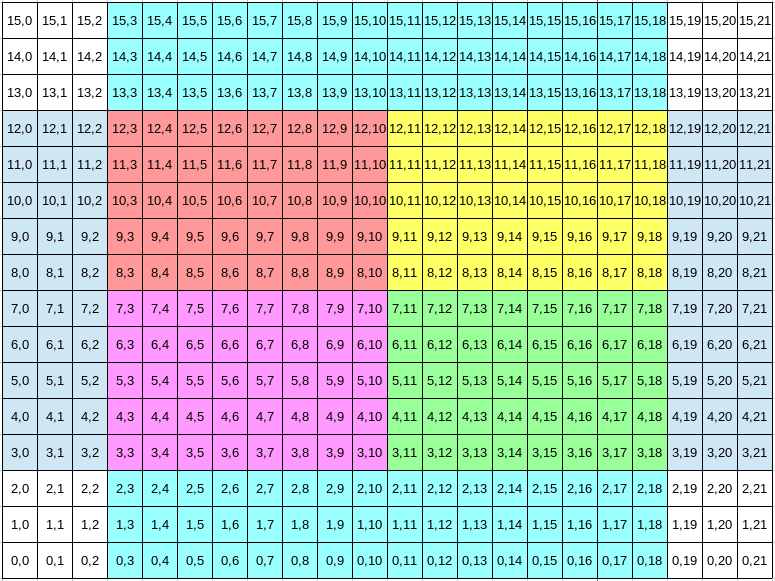
\includegraphics[width=1.0\linewidth]{fig/16x10compDomain}
  \caption{Representation of figure~\ref{fig:ovrvw:mesh} in the computational domain with its extrapolated ghost cells (number of layers = 3) partitioned into 4 as an example.}\label{fig:code:compDom}
\end{figure}

\begin{figure}[!htb]
  \centering
  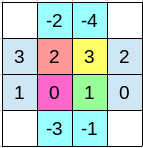
\includegraphics[width=0.175\linewidth]{fig/partition}
  \caption{MPI\_Cart Cartesian communicator setup for 4 partitions referencing the physical, and computational grid in figures~\ref{fig:ovrvw:mesh}, and~\ref{fig:code:compDom}, respectively.}\label{fig:code:part}
\end{figure}

\begin{minted}{cpp}
  MPI_Comm_size(MPI_COMM_WORLD, &size)
  int cnt = size;
  int n = 0;
  while (cnt >= 2){
    cnt = cnt/2;
    n++;
  }
  nj = pow(2, (n/2)); // partitions in the vert direction
  ni = pow(2, (n/2)+n%2); // partitions in the horiz direction
\end{minted}

Currently the number of partitions requested has to be a power of 2, but will be revisited. With the number of partitions in the i and j known the new communicator can be created through

\begin{minted}{cpp}
  int dim[2] = {nj, ni};        // 2 int array for MPI_Cart_Create
  int reorder = FALSE;          // Reorder for fastest comm
  int period[2] = {FALSE, TRUE};// periodic boundary partit

  MPI_Comm com2d; // Setup cartesian communicator
  MPI_Cart_create(MPI_COMM_WORLD, 2, dim, period, reorder, &com2d);
  MPI_Comm_rank(com2d, &rank);
\end{minted}

, where \href{https://www.mpich.org/static/docs/v3.2/www3/MPI\_Cart\_create.html}{MPI\_Cart\_Create} creates a grid of the partitions with periodic capabilities. With the number of partitions in i and j set rank 0 fetches the data from the mesh file currently created using MATLAB. With the coordinates that define the cell known the ghost cell coordinates are extrapolated from the interior, and the areas, normal vectors, and volumes of the cells are then computed which looks like

\begin{minted}{cpp}
if(rank == 0){
  RowMajorMatrixXd xn, yn; // vertices/node coord
  RowMajorMatrixXd xc, yc; // cell center coord
  inputMesh(xn, yn, xc, yc, mesh);// fill coords
  ...
  // extrapolate coordinates for ghost cells
  extrapCopyCoords(xc_g, yc_g, xc, yc, C);
  ...
  // compute geometry note horizontal (i) and vertical (j) dir
  computeArea(Ai, Aj, xn, yn);
  computeNormalVectors(nix, niy, njx, njy, xn, yn, Ai, Aj);
  computeVolume(Volume, xn, yn);
\end{minted}
. Note that rank 0 computes these quantities globally for the entire domain like in figure~\ref{fig:code:compDom} into the RowMatrixXd class which is defined as
\begin{minted}{cpp}
typedef Matrix<double,Dynamic,Dynamic,RowMajor> RowMajorMatrixXd;
\end{minted}
, where using this row major memory storage format allows for easy incorporation with MPICH. With all global geometry defined it is then sent to the other ranks by first sending the size it expects to receive in $nb$

\begin{minted}{cpp}
  int nx = xc.cols();
  int ny = xc.rows(); 
  int nxb = nx/ni; // nx per partition
  int nyb = ny/nj; // ny per partition
  
  nb[0] = nxb;
  nb[1] = nyb;
  for(int r = 1; r < size; r++)
    MPI_Send(nb, 2, MPI_INT, r, 999, com2d);
\end{minted}
, and then the arrays can be sent using the eigen block command 
\begin{minted}{cpp}
// loop over all ranks
for(int j = 0; j < nj; j++){
  for(int i = 0; i < ni; i++){
    int r = j*ni+i; // current rank
    if (r >= 1){ // mpi send
      //block(row start, col start, rows, cols)
      temp = xcg.block(nyb*j, nxb*i, nybg, nxbg); 
      MPI_Send(temp.data(), nxbg*nybg, MPI_DOUBLE, r, 111, com2d);
      ...
    }
    else{ // rank 0 fills its own local geo
      xcLg = xcg.block(nyb*j, nxb*i, nybg, nxbg);
      ...
    } 
\end{minted}
. All the data then has been sent from rank 0 and now is received through

\begin{minted}{cpp}
if(rank == 0){
  ...
}
else{
  int source = 0;
  MPI_Status status;
  // receive sizes
  MPI_Recv(&nb, 2, MPI_INT, source, 999, com2d, &status); 
  ...
  // receive directly into eigen array
  MPI_Recv(xcLg.data(), nxbg*nybg, MPI_DOUBLE, source, 111, com2d, 
    &status);
  ...
}
\end{minted}
. With all the geometry locally defined the only other MPI function needed is for halo exchange/boundary conditions. The next function from algorithm~\ref{fig:alg} is the initialize function which initializes the primitive variables.

\subsection{Initialization \& Time Step}\label{sec:code:init}

After mesh reading the conserved variables are resized in memory based on the geometry from mesh read. The conserved variables are initialized through from the primitive form $\mathbf{Q}=\left[\rho, \mathbf{u}, P, \mathbf{b}\right]^T=\mathbf{V}$ and is done using the initialize function given by
\begin{minted}{cpp}
void initialize(
    Map2Eigen* V,                  // output - Primitive variables 
    const RowMajorMatrixXd& xc_g,  // input - xcoord with ghosts cells
    const RowMajorMatrixXd& yc_g,  // input - ycoord with ghosts cells
    constants C){                  // input - constants for case number
\end{minted}
. Note Map2Eigen is a wrapper that sets up a 3 dimensional array that is mapped to a single C array set up in row major format like
\begin{minted}{cpp}
U->Q_raw = {rho, u, v, w, p, bx, by, bz, rho, u, v, ...}
U->Q[rhoid](j, i) = rho
U->Q[uid](j, i) = u 
U->Q[vid](j, i) = v
...
\end{minted}
. Using this map allows for the structure of the serial code to not be altered while being MPI compatible. For the MRT test case the initialized values are based off of the \href{https://www.astro.princeton.edu/~jstone/Athena/tests/rt/rt.html}{Athena Webpage} and are given by
\begin{minted}{cpp}
  double rhoL=1.0;
  double rhoH=1.0;
  double P0=2.5;
  double B=0.125
  double g=0.1;
\end{minted}
, where all units are unitless through normalized quantities. Note that numerical values are given above, but in the code global variables are used and are defined from the input file. $\mathbf{V}$ is then assigned by
\begin{minted}{cpp}
  for(int j = 0; j < nj; j++){
    for(int i = 0; i < ni; i++){
      ...
      //compute radius and angle
      double r = sqrt(x*x + y*y); 
      double thet = atan2(y,x);
      //fill density
      if(r < rMiddle)
        V->Q[rhoid](j,i)=rhoL; // fill light fluid
      else
        V->Q[rhoid](j,i)=rhoH; // fill heavy fluid
      ...
\end{minted}
, for brevity only the initialization of density is shown see code "parr/src/mhd\_f.cpp" for full details. This function is written so that any rank can initialize its own primitive variables based on its coordinates of cell centers, so there is no MPI code needed. Next would be time step, but it simply uses the fastest wave speed (fast magnetosonic speed) and an averaging based on areas, normal vectors, and volumes; see "parr/src/mhd\_f.cpp" for details. Once each rank has computed its local minimum time step an all reduce command is used to set the time step on all ranks and is done in the main file by

\begin{minted}{cpp}
  ...
  dt = computeTimeStepU(Volume, Ai, Aj, nix, niy, njx, njy, U, C);
  MPI_Allreduce(MPI_IN_PLACE, &dt, 1, MPI_DOUBLE, MPI_MIN, com2d);
  ...
\end{minted} 

\subsection{Halo Exchange \& Boundary Conditions}
Every partition for this code must send its ghost cell layer $\mathbf{Q}$'s to its neighboring partitions unless it is a physical boundary. Periodic physical boundaries are used for the left and right walls, while a perfectly conducting wall is used for the top and bottom walls. The function that does these operations is
\begin{minted}{cpp}
void mpiSetBc(
    Map2Eigen* U,                 //Out: conserved vars
    const RowMajorMatrixXd& nix,  //In: norm vec xcomp i dir
    const RowMajorMatrixXd& niy,  //In: norm vec ycomp i dir
    const RowMajorMatrixXd& njx,  //In: norm vec xcomp j dir
    const RowMajorMatrixXd& njy,  //In: norm vec ycomp j dir
    MPI_Comm& com2d,              //In: Communicator 
    constants C){
\end{minted}
. With the cartesian MPI communicator nearest neighboring partitions are found using \href{https://www.mpich.org/static/docs/v3.2/www3/MPI_Cart_shift.html}{MPI\_Cart\_Shift} of which internally keeps track of physical walls ($-$ number), and periodic walls
\begin{minted}{cpp}
int r, l, u, d;
int rank;
MPI_Comm_rank(com2d, &rank);
//MPI_Cart_Shift(communicator, direction, displacement, source, dest)
MPI_Cart_shift(com2d, 0, 1, &d, &u); 
MPI_Cart_shift(com2d, 1, 1, &l, &r);
\end{minted}
. Applying as an example partition 3 in figure~\ref{fig:code:part} will have left $=$ 2, right $=$ 2, down $=$ 1, and up $=$ -4. With the nearest neighbors of every partition known apply boundary conditions/halo exchange for all boundaries. The left and right boundaries are periodic (with the exception of x and y component quantities of $\mathbf{Q}$), and to send the data 
\begin{minted}{cpp}
int sendSize = njc*C.num_ghost*NEQ; // njc number of rows with ghost
Map2Eigen *tempLout = new Map2Eigen(njc , C.num_ghost, NEQ);
int ic = C.num_ghost;
int sign = +1;
for(int i = 0; i < C.num_ghost; i++)
  for(int eq = 0; eq < NEQ; eq++)
    tempLout->Q[eq].col(i) = U->Q[eq].col(ic+sign*i);
if(l>rank){
  // flip sign for phys periodic boundary
  tempLout->Q[uid]  =-1.0*tempLout->Q[uid];
  tempLout->Q[vid]  =-1.0*tempLout->Q[vid];
  tempLout->Q[bxid] =-1.0*tempLout->Q[bxid];
  tempLout->Q[byid] =-1.0*tempLout->Q[byid];
}
// sent to left 
int tag = 222; // right recv
int out = l;
MPI_Isend(tempLout->Q_raw, sendSize, MPI_DOUBLE, out, tag, 
  com2d, &requestOut[0]);//tag222 is right
\end{minted}
for the left which can similarly be done for the right. The upper and lower surface physical boundary is a perfectly conducting wall so that the normal component of $\mathbf{u}$, and $\mathbf{b}$, is $0$ at the wall, and with normal vectors are given by
\begin{align*}
  u_g &= -n_x(u n_x + v n_y) - n_y(-u n_y + v n_x)\\
  v_g &= -n_y(u n_x + v n_y) + n_x(-u n_y + v n_x)\\
  b_{xg} &= -n_x(b_x n_x+b_y n_y) - n_y( -b_x n_y + b_y n_x)\\
  b_{yg} &= -n_y(b_x n_x + b_y n_y) + n_x(-b_x n_y + b_y n_x)
\end{align*}
, where $u,v,b_x,b_y$ are the interior cell values. The other quantities in $\mathbf{Q}$ ($\rho, \rho w, \epsilon, b_z$) are extrapolated from the interior through
\begin{minted}{cpp}
  sendSize = nic*C.num_ghost*NEQ;
  Map2Eigen *tempBout  = new Map2Eigen(C.num_ghost, nic, NEQ);
  int jfo = 0;// bottom face
  int jco = C.num_ghost; // bott inter offset
  int jgo = C.num_ghost - 1; // ghost start bott
  int sign = +1;// direction to push
  if(d < 0){// phys bndry conducting wall
    for(int j = 0; j < C.num_ghost; j++)
      for(int i = C.num_ghost; i < nic-C.num_ghost; i++){
        int iff = i - C.num_ghost;// index for normvecs
        int jc = jco + sign*j; // cell interior
        int jg = jgo - sign*j; // ghost cell row-layer
        ...
        // bottom boundary no penetration conducting wall
        U->Q[uid](jg,i) = -nx*(u*nx+v*ny) - ny*(-u*ny + v*nx);
        U->Q[vid](jg,i) = -ny*(u*nx+v*ny) + nx*(-u*ny + v*nx);
        ... //bxid byid
        // extrapolate from cells in sign dir
        U->Q[rhoid](jg,i) = 2.0*U->Q[rhoid](jg+sign*1,i) 
          - U->Q[rhoid](jg+sign*2,i);
        ... //pid bzid wid
      }
  }
  else{ // not phys bndry
    // send bott dat
    out = d;
    tag = 444; //tag444top receive
    for(int j = 0; j < C.num_ghost; j++)
      for(int eq = 0; eq < NEQ; eq++)
        tempBout->Q[eq].row(j) = U->Q[eq].row(jco+sign*j);
    MPI_Isend(tempBout->Q_raw, sendSize, MPI_DOUBLE, out, tag, 
      com2d, &requestOut[2]); 
  }
\end{minted}
, and similarly for the top boundary. Now each rank has either applied its boundary conditions, or sent its data to be received by the neighboring rank. The receives for the left and bottom are given by
\begin{minted}{cpp}
  Map2Eigen *tempLin  = new Map2Eigen(njc , C.num_ghost, NEQ);
  sendSize = njc*C.num_ghost*NEQ;
  in = l;
  tag = 111;
  ico = C.num_ghost;//left inter offset
  sign = +1;
  MPI_Irecv(tempLin->Q_raw, sendSize, MPI_DOUBLE, in, tag, com2d,
    &requestIn);
  MPI_Wait(&requestIn, &status);
  for(int i = 0; i < C.num_ghost; i++)
    for(int eq = 0; eq < NEQ; eq++)
      U->Q[eq].col((ico-1)-sign*i) = tempLin->Q[eq].col(i);
  ...
  if (d >= 0){
    Map2Eigen *tempBin  = new Map2Eigen(C.num_ghost, nic, NEQ);
    sendSize = C.num_ghost*nic*NEQ;
    in = d;
    tag = 333;
    jco = C.num_ghost; // bott inter offset
    sign = +1;
    MPI_Irecv(tempBin->Q_raw, sendSize, MPI_DOUBLE, in, tag, com2d, 
      &requestIn); //tag444top
    MPI_Wait(&requestIn, &status);
    for(int j = 0; j < C.num_ghost; j++)
      for(int eq = 0; eq < NEQ; eq++)
        U->Q[eq].row(jco-1-sign*j) = tempBin->Q[eq].row(j); 
  }
  ...
\end{minted}
. Refer to "parr/src/mhd\_f.cpp" for other functions such as MUSCL, source term, 2D flux, Residual, and RungeKutta, as these functions where not something developed in this course and are omitted for brevity. Though the 2D flux function has been expanded for the MHD equations, the functional form is outlined in section~\ref{sec:disc} and follows similarly to the work done already in the serial code.

\subsection{GPU}
Coding for the GPU consisted of only modifying the non MPI functions such as MUSCL, source term, 2D flux, Residual, and Runge Kutta. Kernels were written for each, and only a couple will be highlighted in detail. The Residual function was changed to

\begin{minted}{cpp}
@kernel void computeRes(double* Res,
        const double* S,
        const double* F,
        const double* G,
        const double* Aj,
        const double* Ai,
        const double* Volume)
{
  for (int j = 0; j < o_njc; j++;  @tile(8, @outer, @inner)){
    for (int i = 0; i < o_nic; i++; @tile(32, @inner)){
      // res = right + top - left - bottom - source
      const int nj = o_njc;
      const int ni = o_nic;
      const int idl = (j*(ni+1)+i);
      const int idr = (j*(ni+1)+i+1);
      const int idb = (j*ni+i);
      const int idc = (j*ni+i);
      const int idt = ((j+1)*ni+i);

      for (int eq = 0; eq < o_NEQ; eq++){
        Res[idc*o_NEQ+eq] = F[idl*o_NEQ+eq]*Ai[idl]
          + G[idb*o_NEQ+eq]*Aj[idb]
          - F[idr*o_NEQ+eq]*Ai[idr]
          - G[idt*o_NEQ+eq]*Aj[idt]
          - S[idc*o_NEQ+eq]*Volume[idc];
      }
    }
  }
}
\end{minted}
. Another example is from computeSourceTerm which is

\begin{minted}{cpp}
@kernel void computeSourceTerm(
        double* S, 
        @restrict const double* U, 
        @restrict const double* xc, 
        @restrict const double* yc){
  for(int j = 0; j < o_njc; j++;@tile(8, @outer, @inner))
  {
    for(int i = 0; i < o_nic; i++; @tile(32, @inner))
    {
      int jg = j + o_ng;
      const int ig = i + o_ng;
      const int fill = j*o_nic+i;
      const double rho = U[(jg*o_nic_g+ig)*o_NEQ+o_rhoid];
      const double thet = atan2(yc[j*o_nic+i], xc[j*o_nic+i]);
      const double su = -1*(rho)*(o_ACCEL)*cos(thet);
      const double sv = -1*(rho)*(o_ACCEL)*sin(thet);
      // Need to take advantage of contiguous memory revisit later
      S[(fill)*o_NEQ+o_piid]= ((su*(-1)*o_ACCEL*cos(thet)) 
        + (sv*(-1)*o_ACCEL*sin(thet)));
      S[(fill)*o_NEQ+o_uid] = su;
      S[(fill)*o_NEQ+o_vid] = sv;
    }        
  }           
}
\end{minted}
. Note that these kernels need to be optimized in many ways, and achieve low-medium dram efficiency, and low flop utilization.

\section{Performance \& Results}
The widely known classical linear growth rate for the RT instability is $\gamma = \sqrt{A g k}$ where $A$ is the Atwood number, $g$ is the acceleration, and $k$ is the wavevector. The growth rate can be used to identify an end time where sufficient MRT growth can be observed. Using the initialized values from \ref{sec:code:init}, and running to 1 inverse growth with 10\% velocity gained perturbation ($g*tend*10\%$) results in Figure~\ref{fig:res:base}. All simulations used a mesh size of 560x480, and were run with mpi using 16 processors except for the GPU which was serial. From Figure~\ref{fig:res:base} there could be an issue with the Halo exchange that is causing the broken segment at the middle radius, or an issue with the initial perturbation being too large. Though if it were in the halo exchange it would have appeared in Figure~\ref{fig:res:5g} where the acceleration is increased 5 fold. As expected with larger acceleration there will be larger growth at the same end time. With magnetic fields properly aligned tangent to the interface they can help stabilize against the MRT instability this is observed in Figures~\ref{fig:res:10bx}\&~\ref{fig:res:50bx} where the interface is halted due to large magnetic field. Note that this algorithm has no divergence cleaning/correction, so $\nabla\cdot\mathbf{b}\neq0$ which can be cleaned through diffusion and advection. Figure~\ref{fig:res:gpu} shows the result of a reduced perturbation, as well as being run on a GPU, and the reduced perturbation shows less shocks within the heavy and light medium.

The performance of the MPI \& GPU code is summarized in Figures~\ref{fig:res:mpi}~\&~\ref{fig:res:roof} showing MPI scaling, and roofline modeling, respectively. The MPI scaling was done on one node, and showed factor of 2 speed up through the max of 16 processors, when moving to multiple nodes there was a significant slow down as expected (for 32 processors elapsed time went from \SI{40}{sec}$\rightarrow$\SI{40}{sec}). Figure~\ref{fig:res:roof} shows the intensity of the kernels vs the FLOPS utilized, and clearly the code is not very optimized. Further development is required to increase the performance of these kernels such as better utilization of shared memory. 

\begin{figure}[!htb]
  \centering
  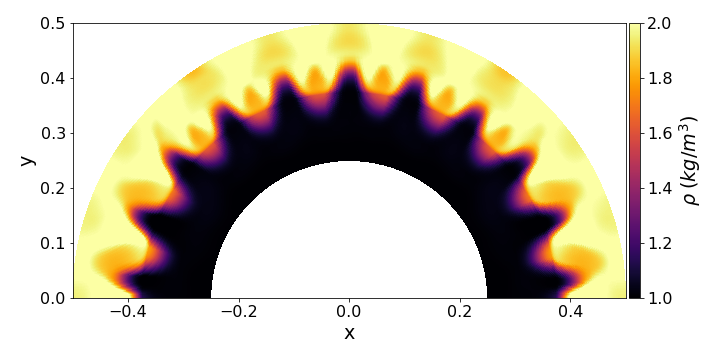
\includegraphics[width=1.0\linewidth]{fig/560x480cpuBase}
  \caption{Shows density growth at \SI{0.12891}{}}\label{fig:res:base}
\end{figure}
\begin{figure}[!htb]
  \centering
  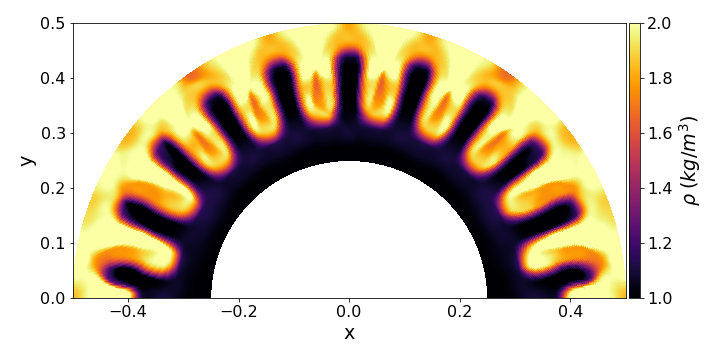
\includegraphics[width=1.0\linewidth]{fig/560x480cpu}
  \caption{Shows density growth at \SI{0.12891}{} with 5$g$}\label{fig:res:5g}
\end{figure}

\begin{figure}[!htb]
  \centering
  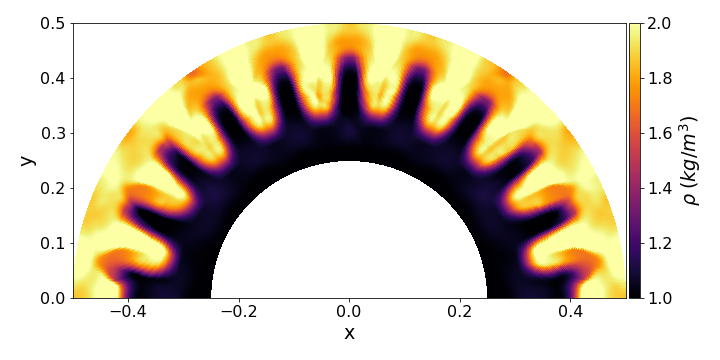
\includegraphics[width=1.0\linewidth]{fig/560x480cpuBx}
  \caption{Shows density growth at \SI{0.12891}{} with 5$g$ and 10$B_t$}\label{fig:res:10bx}
\end{figure}
\begin{figure}[!htb]
  \centering
  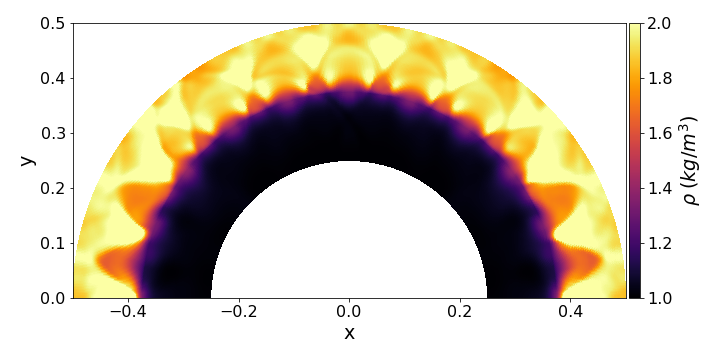
\includegraphics[width=1.0\linewidth]{fig/560x480cpuBx5}
  \caption{Shows density growth at \SI{0.12891}{} with 5$g$ and 50$B_t$}\label{fig:res:50bx}
\end{figure}

\begin{figure}[!htb]
  \centering
  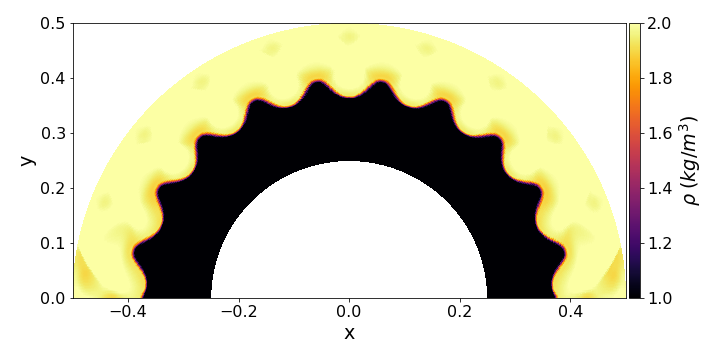
\includegraphics[width=1.0\linewidth]{fig/560x480gpu}
  \caption{Shows density growth at \SI{0.12891} using a perturbation of 5\%}\label{fig:res:gpu}
\end{figure}

\begin{figure}[!htb]
  \centering
  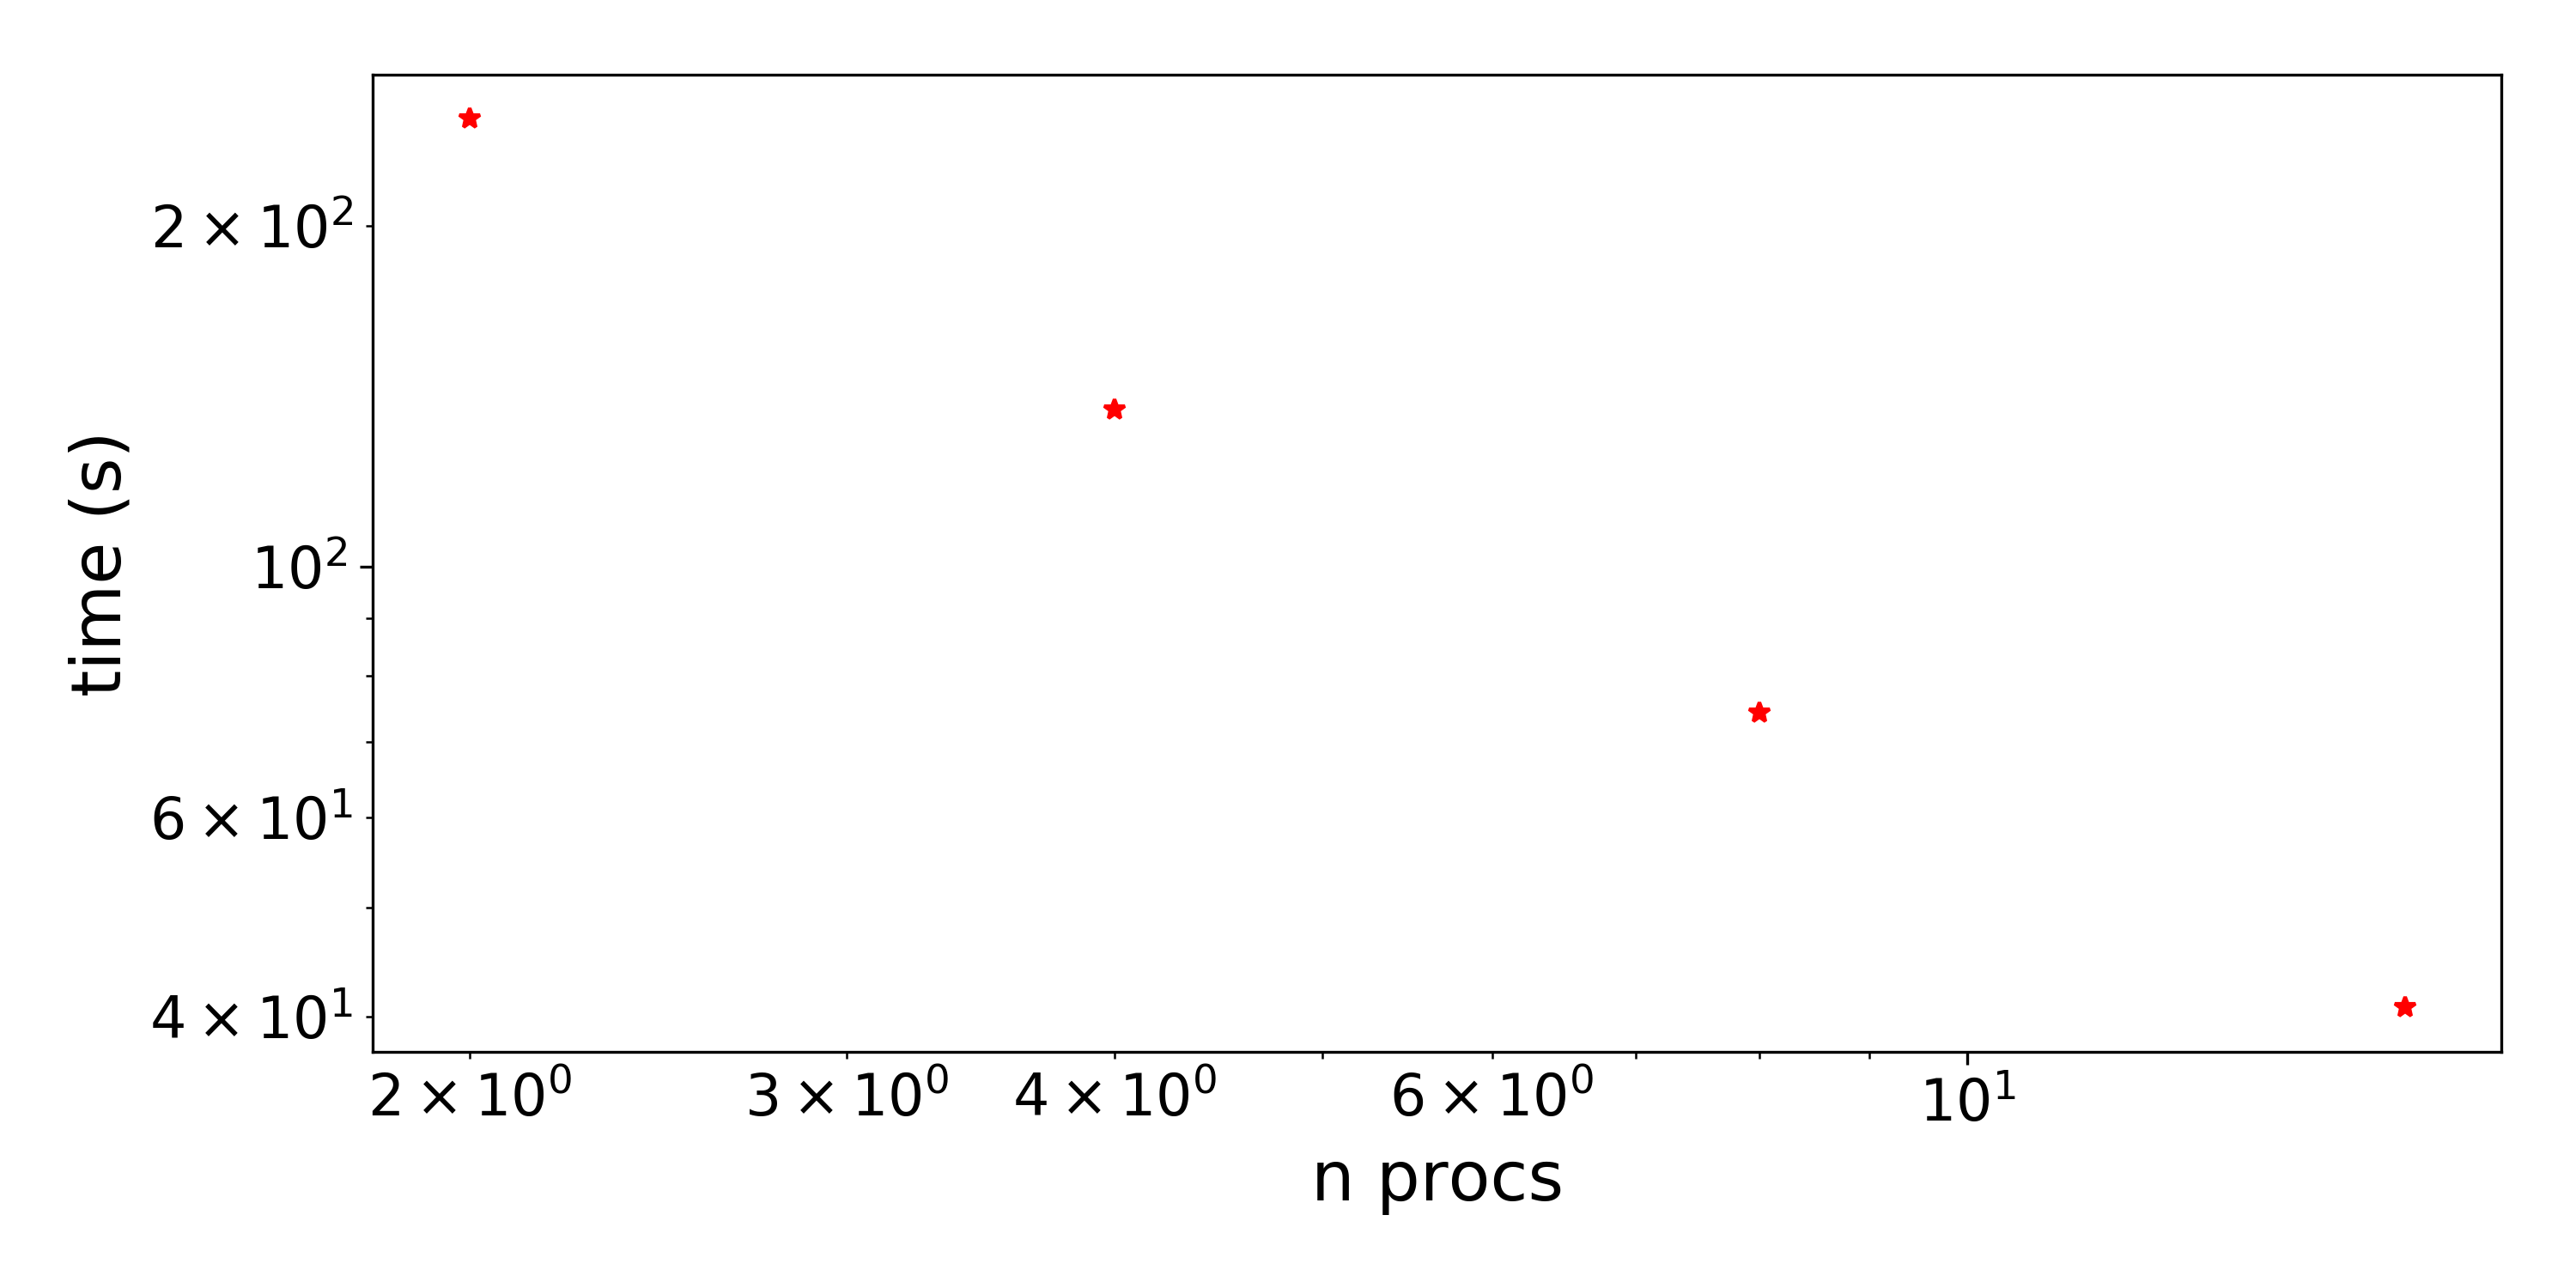
\includegraphics[width=1.0\linewidth]{fig/mpiScaling}
  \caption{MPI scaling on a fixed grid size of 360x300 and a fixed end time of \SI{0.12891}{}}\label{fig:res:mpi}
\end{figure}

\clearpage
\begin{figure}[!htb]
  \centering
  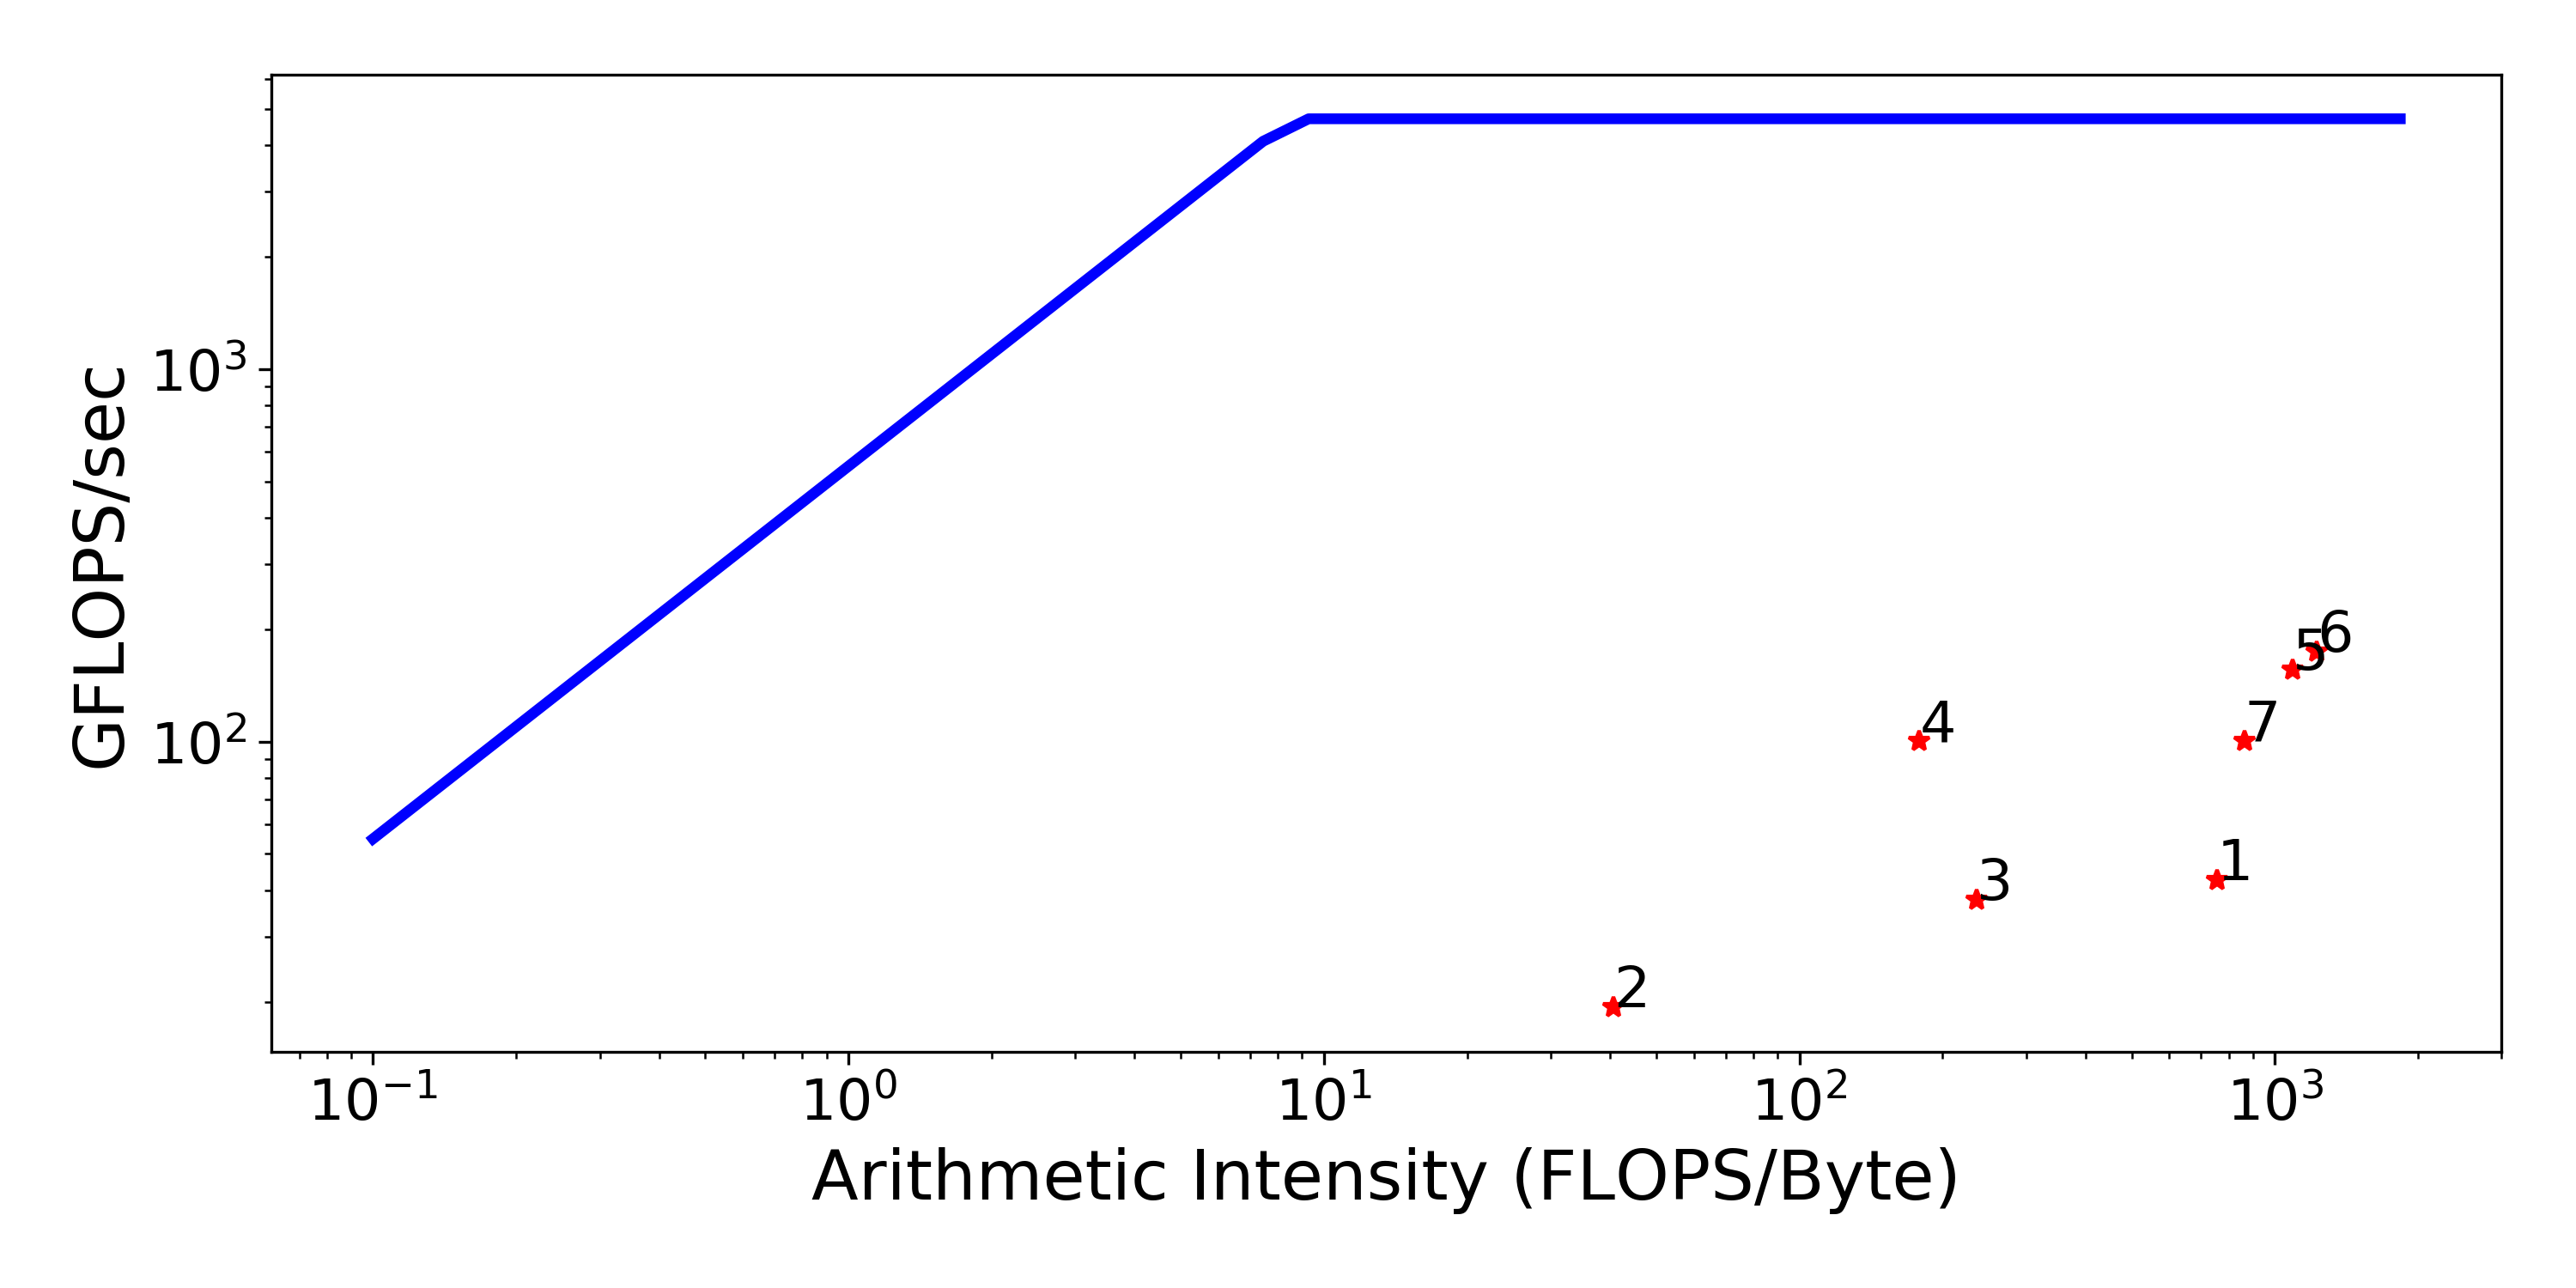
\includegraphics[width=1.0\linewidth]{fig/rooflinemodeling}
  \caption{Roofline modeling showing the different kernels with 1, 2, 3, 4, 5, 6, 7, representing source term, residual, Runge Kutta, MUSCL LR, 2D Flux F, 2D Flux G, and MUSCL BT, respectively.}\label{fig:res:roof}
\end{figure}

\section{Summary}

The work done to parallelize, solve a new set of equations, and utilize GPU explored many new features available such as MPI\_Cartesian communicator, Eigen matrix mapping, etc.. Additional ARS were explored but not successfully implemented (see "src/mhd\_f.cpp") such as the Powell 8 wave ARS \cite{powell1994}, and the Miyoshi HLLD 5 wave ARS \cite{miyoshi2005}. Overall The code showed some physically relevant results, but still requires verification and validation. Some validation testing can be energy conservation, and divergence free checking of $\mathbf{b}$; some verification testing can be method of manufactured solutions \cite{roy2005}. There are still some discrepancies in the results, and there are likely bugs in the end code, but MPI scaling shows promising strong scalability. Additionally optimization of the GPU code needs to be explored due to low performance, and the steps made in class would be a starting point. 

\clearpage
 \bibliographystyle{IEEEtran}
  \bibliography{reference}
%%% End document
\end{document}
